\documentclass[a4paper, 12pt, english]{article}
\usepackage[utf8]{inputenc}
\usepackage{fancyhdr}
\usepackage{graphicx}
\usepackage{lastpage}
\usepackage{layout}
\usepackage{enumitem}
\usepackage{etoolbox}
\usepackage{amsmath}
\usepackage{mathptmx}
\usepackage[bottom]{footmisc}
\usepackage[includeheadfoot, left=3cm, right=3cm, top = 1.5 cm]{geometry}
\usepackage{minted}
\usemintedstyle{xcode}


\graphicspath{ {./answers/} }

\pagestyle{fancy}
\fancyhf{} 
\rhead{
    {\Large \textbf{Analysis and Design of Algorithms}}\\
    \textbf{CS2102} \\ 
    \textbf{Divide and Conquer Practice} \\ 
    \textbf{2020-II}
}
\lhead{
\includegraphics[width=4.6cm, keepaspectratio]{logo/utec}}
\rfoot{\textbf{\thepage}\hspace{1pt} of \textbf{\pageref{LastPage}}}
\cfoot{}

\setlength{\parindent}{0em}
\setlength{\headheight}{80pt}

\newcounter{problem}[section]
\newenvironment{problem}[3][]{\refstepcounter{problem}\par\medskip 

\textbf{Problem~\theproblem  ~~(#2) - 
\ifboolexpr{
  test {\ifdimless{1 pt}{#3 pt}}
}
{#3 points} % true
{#3 point} % false
} \newline\newline } {\medskip} 

\usepackage{pdfpages}
\begin{document}

\textbf{Submission deadline}: 14 Nov, 23:59\\ 

\begin{itemize}
    \item Write your answers(images) and C++ code inside the \emph{answers} folder in order to generate a single PDF file. Replace the images and cpp files that are already included in the project. Do not change the file name.
    \item Read the questions carefully and write your answers clearly. Answers that are not legible and that doesn't follow the format will not have any score. 
\end{itemize}

\underline{Outcomes}:

\begin{enumerate}[label=\alph*.]
    \item Apply appropriate mathematical and related knowledge to computer science.
    \item Analyze problems and identify the appropriate computational requirements for its solution.
\end{enumerate}
\noindent\rule{\textwidth}{0.01pt}
\vspace{3mm}

\section{Warm up}

\begin{multicols}{2}[\columnsep1em] 
    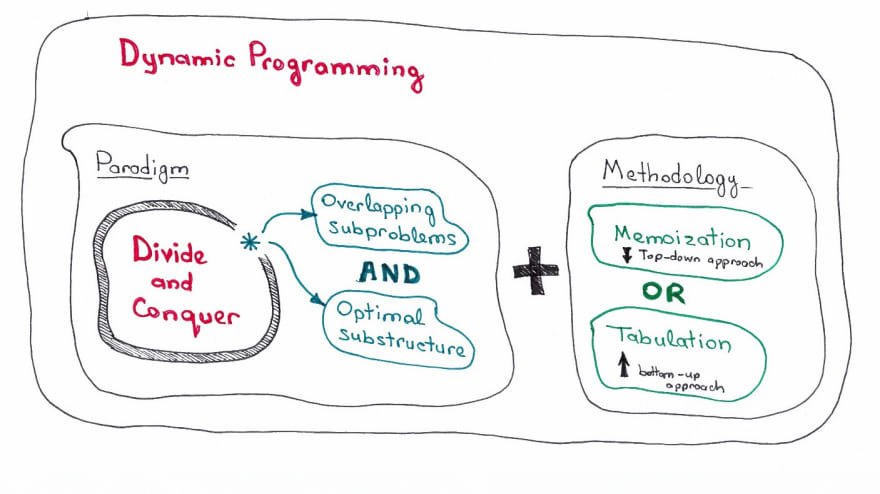
\includegraphics[width=\linewidth]{img/dynamic}
    \columnbreak

    In the previous lecture we presented 2 approaches to store the results of subproblems that are progressively used to construct the final solution to a particular problem:
    \begin{itemize}
        \item Memoization ( top-down approach )
        \item Tabulation ( bottom-up approach )
    \end{itemize}
\end{multicols}

\begin{problem}{Outcome b}{4}
    Remember the idea behind the top-down approach and 
    for each of the following items implement 2 algorithms in C++, 
    one with the regular recursive implementation and the other using the memoization approach:

    \begin{itemize}
        \item Fibonacci function
            \inputminted[fontsize=\small,breaklines]{cpp}{answers/problem1/problem1-1.cpp}
        \item Factorial function
            \inputminted[fontsize=\small,breaklines]{cpp}{answers/problem1/problem1-2.cpp}
    \end{itemize}
\end{problem}

\begin{problem}{Outcome b}{2}
    Answer the following questions:
    \begin{itemize}
        \item What are the differences between the memoization and tabulation approaches? Which one is faster?
        \item What are the main conditions that a problem must present in order to be solvable using dynamic programming? 
            Explain those conditions with the C++ algorithms proposed above.
    \end{itemize}

    \begin{center}
        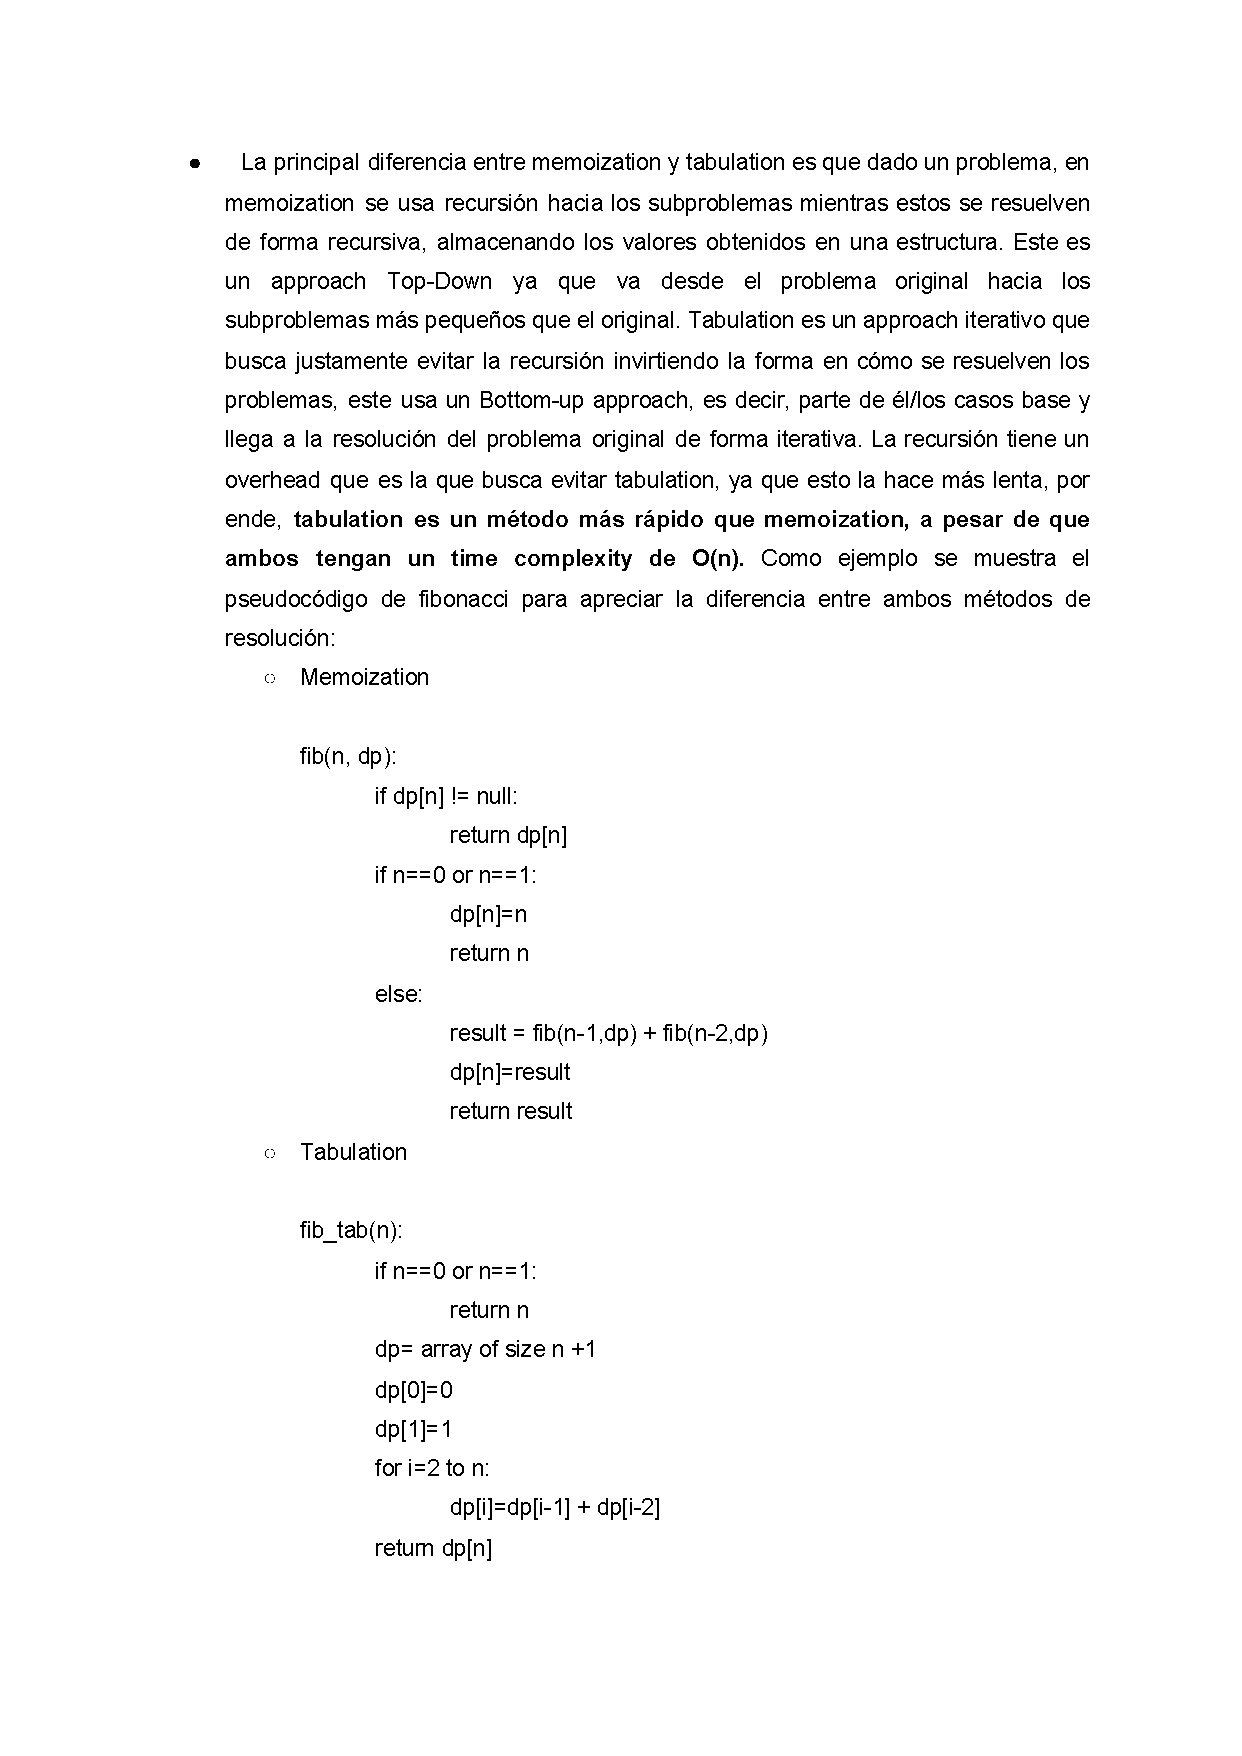
\includepdf[page={1,2}]{answers/problem2/problem2.pdf}
    \end{center}
\end{problem}

\section{Dynamic Programming Problems}

\subsection{0-1 Knapsack Problem}

Given a backpack that can carry $W$ kg and a number of $n$ items where each item has an associate weight($w_{i}$) and value($v_{i}$) we want to know what is the maximum value that we can carry in the backpack. \newline\newline
Consider that if we select any of the items and put it into the backpack we are increasing the total value(\$) but we are decreasing the capacity(kg) of the backpack.

\begin{problem}{Outcome b}{2}
    Consider the items below to calculate the maximum value that we can put into the backpack. 
    \begin{center}
        \begin{tabular}{S|SSSSS} \toprule
            \text{Item}          & 1 $$& 2 & 3  & 4 & 5  \\ \midrule
            \text{Weight (kg)}   & 1 & 2 & 4  & 1 & 12 \\
            \text{Value (\$)}    & 1 & 2 & 10 & 2 & 4  \\ \bottomrule
        \end{tabular}
    \end{center}
    \begin{itemize}
        \item Write down your solution using the tabulation method. ( C++ code shouldn't be attached )
        \item Explain the procedure to get the items that maximize the value in the backpack and write down those items.  
    \end{itemize}


    \begin{center}
        
\includegraphics[width=0.9\linewidth]{problem3/problem3}%
    \end{center}
    
\end{problem}

    
\subsection{Maximum Contiguous Subarray Sum Problem}

Consider the maximum-subarray problem presented in the Chapter 4.1 of the Introduction to Algorithms book.

\begin{problem}{Outcome b}{3}
    Use the rate of change of the daily stock prices presented in the book (Fig. 4.1) to calculate the maximum sum of a contiguous subarray using the tabulation method. ( No C++ code required in this problem )

    \begin{itemize}
        \item Write down the table and the procedure used to solve the problem using dynamic programming.
        \item Once the table is constructed, explain how can we obtain the contiguous subarray given the maximum sum?
    \end{itemize}


    \begin{center}
        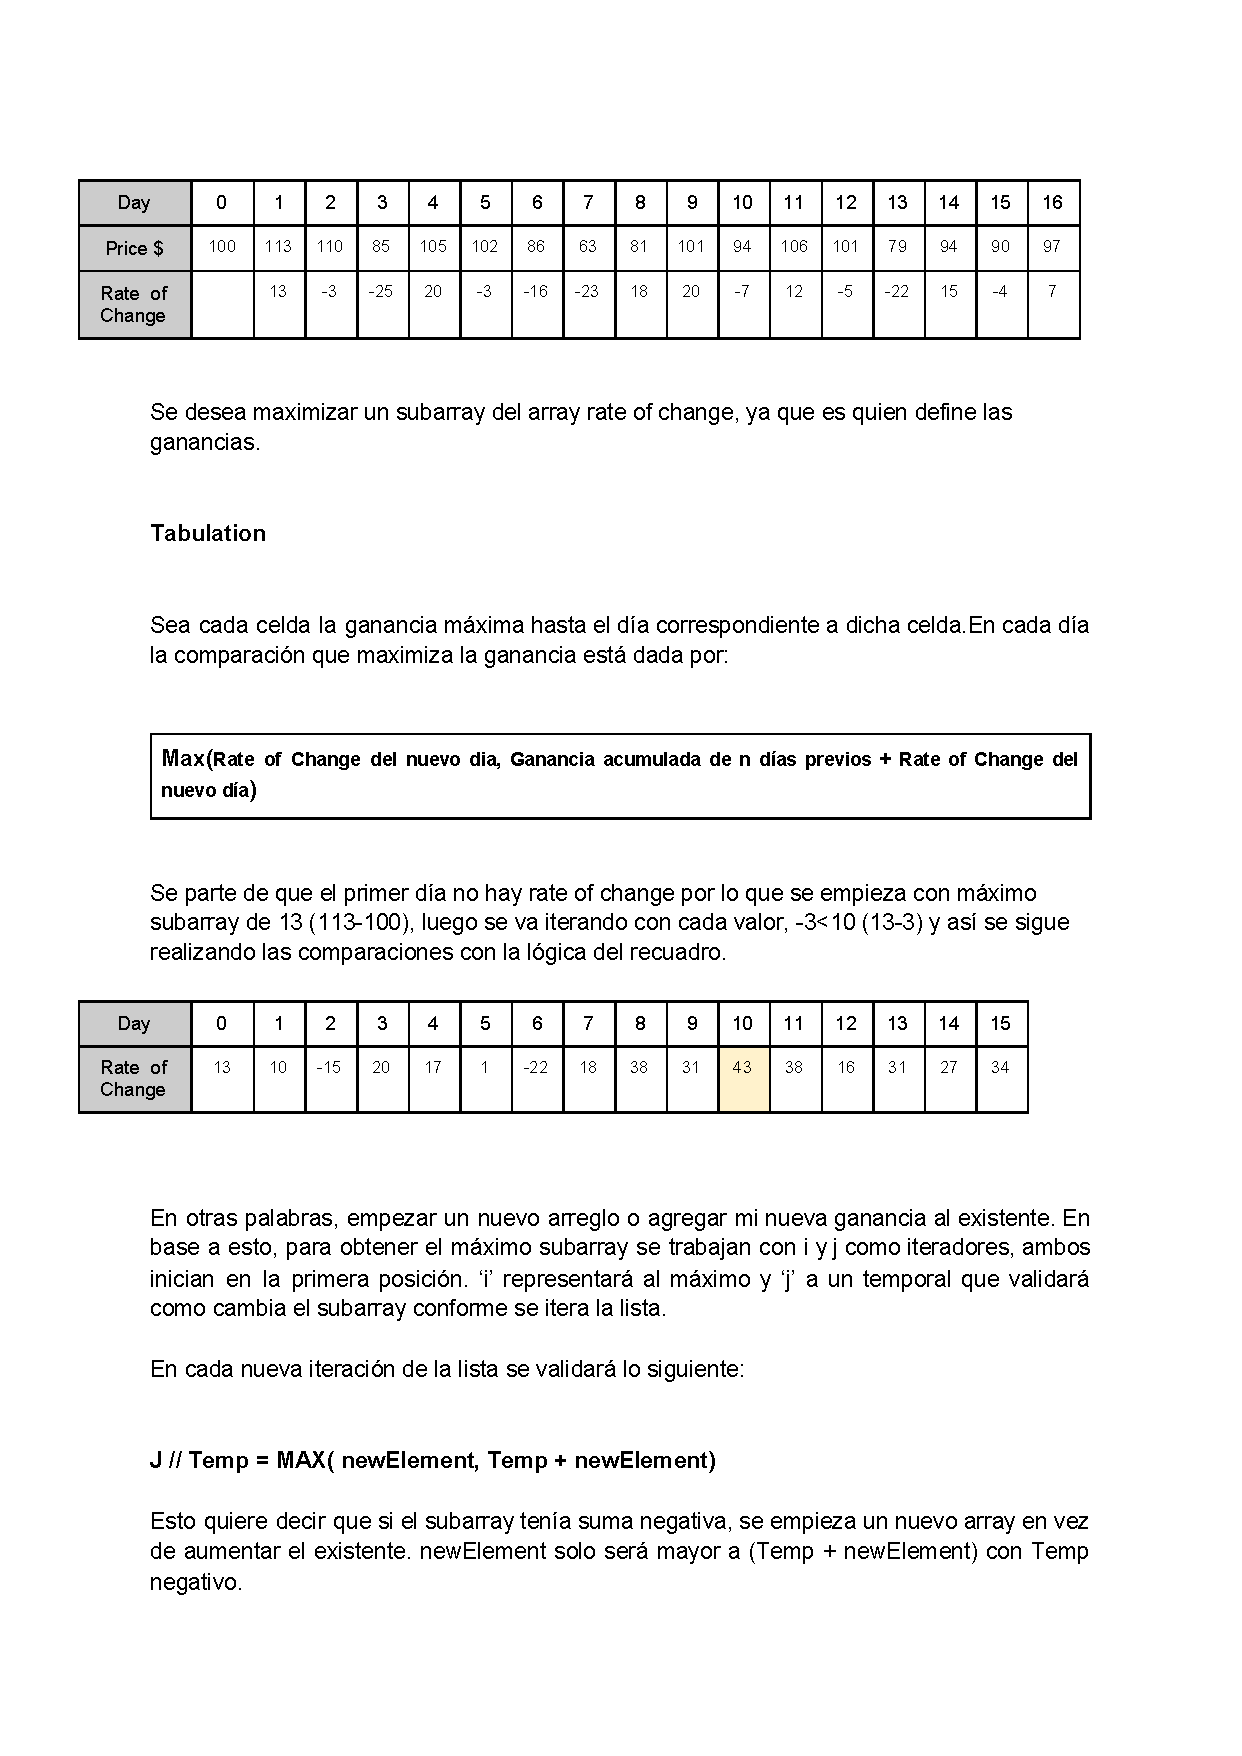
\includepdf[page={1,2}]{answers/problem4/problem4.pdf}
    \end{center}

\end{problem}


\begin{problem}{Outcomes a, b}{6}
    Implement 2 algorithms in C++ to solve the Maximum Contiguous Subarray Sum Problem given an array of positive and negative numbers.
    One algorithm should implement the solution using the Divide and Conquer approach from Chapter 4 
    and the other algorithm should implement a Dynamic Programming bottom-up approach.\newline

    Perform all the trials needed to see the asymptotic behavior of both algorithms considering that the Divide and Conquer approach should behave like a $nlog(n)$ function and the Dynamic Programming algorithm should behave like a linear function.\newline

    \textbf{Recommendations}
    \begin{enumerate}
        \item Implement both algorithms in C++ based on a given array of numbers ( positives and negatives ).
        \item Write a function that given a size it generates a random array of numbers.
        \item Write a function that measures the execution time of an algorithm
        \item Record the execution time of both algorithms given an array of size $k$ and repeat until $k$ is sufficiently large.
        \item Tune your trials and parameters in order to see an smooth execution time similar to the $nlog(n)$ and linear functions.
        \item Attach the source code and generate one picture with both results and attach that image in this problem. 
    \end{enumerate}
    \textbf{Divide and Conquer}
    \inputminted[fontsize=\small,breaklines]{cpp}{answers/problem5/problem5dc.cpp}
    \textbf{Dynamic programming}
    \inputminted[fontsize=\small,breaklines]{cpp}{answers/problem5/problem5dp.cpp}
    Se puede observar en la gáfica un comportamiento O(n lg n) para la versión Divide and Conquer y un comportamiento O(n) para Dynamic programming
    \begin{center}
        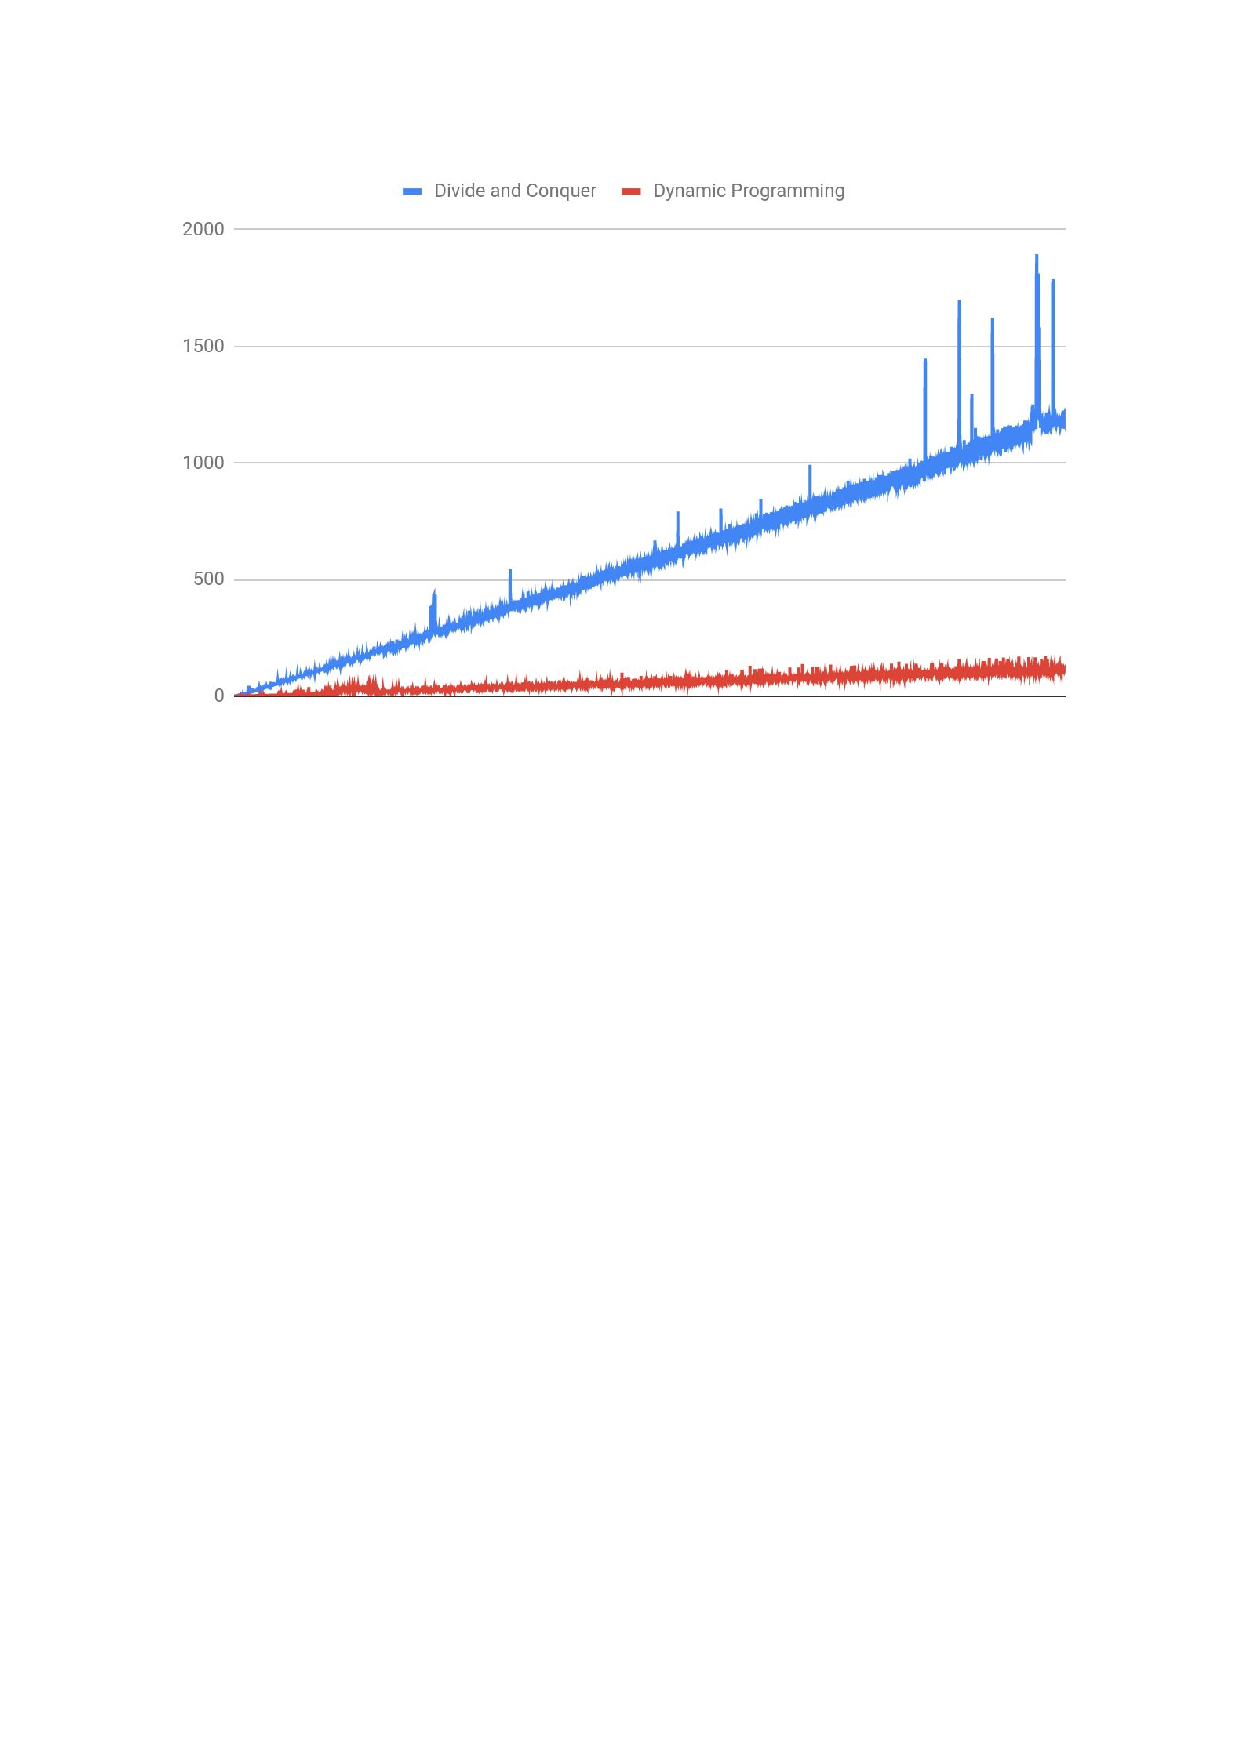
\includegraphics[width=0.9\linewidth]{problem5/problem5.pdf}%
    \end{center}
\end{problem}


\subsection{Coin Change Problem}
Given an amount A and a number of $n$ coins of different denominations the Coin Change Problem ( or at least one variation ) consists in calculate the minimum number of coins that we need to obtain the specific amount. \newline


\begin{problem}{Outcome b}{3}

Consider the following coins and write the table of the tabulation approach considering that the total amount is 18.

\begin{center}
    \begin{tabular}{ |c|c|c|c|c|c|c| } 
        \hline
        \textbf{Coins}  & 1 & 5 & 2 & 6 & 11 & 15 \\ 
        \hline
    \end{tabular}
    \newline
\end{center}

 \begin{center}
    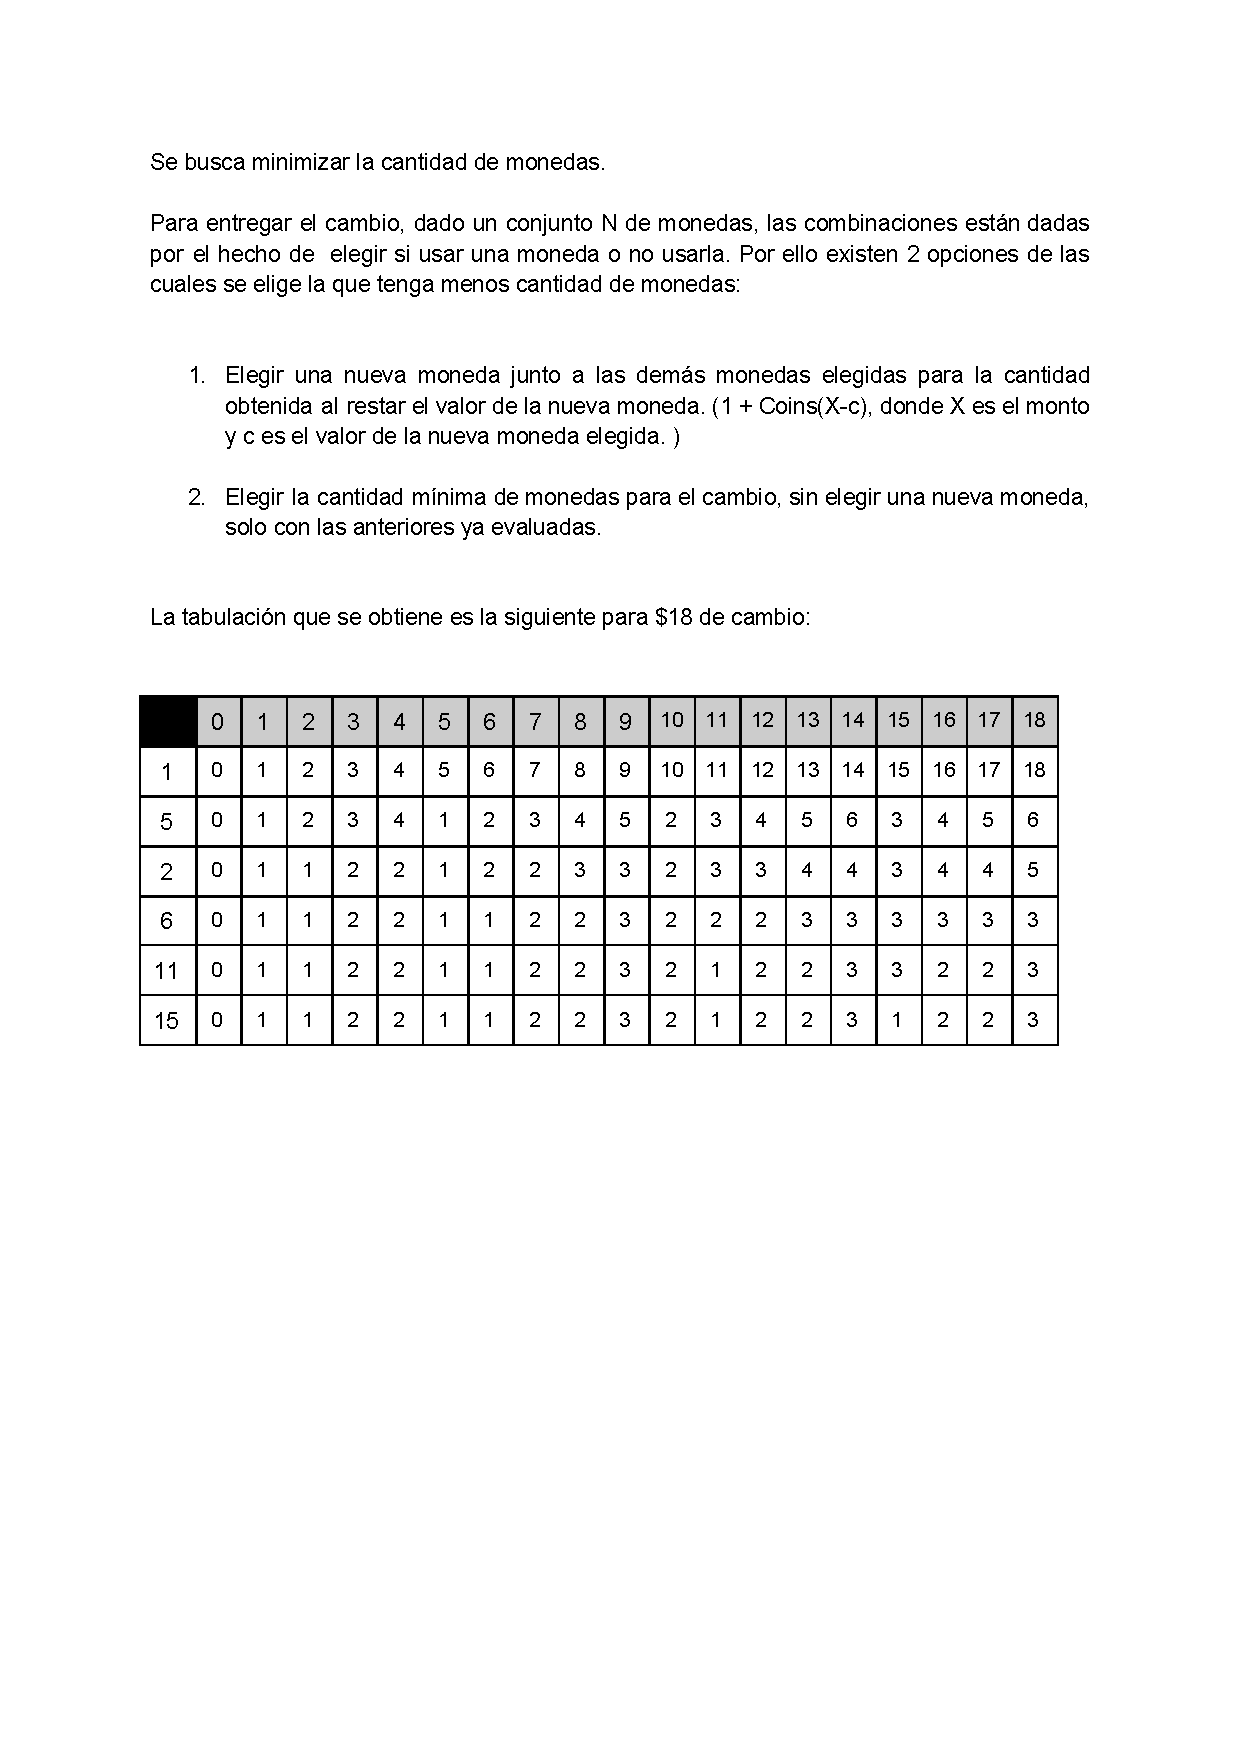
\includegraphics[width=0.9\linewidth]{problem6/problem6}%
\end{center}

\end{problem}
\end{document}



